\lecture{Tue. 9/11/12}
The first problem set is out. Turn in the homework in 2-285.
About homeworks: The optional problems are only for A+'s; we count how many optional problems you solved correctly.

Look at the homework before the day before it's due! The problems aren't tedious lemmas that Sipser doesn't want to do in lectures. He chose them for creativity, the ``aha" moment. They encourage you to play with examples, and don't have overly long writeups. Write each problem on a separate sheet, and turn them in in separate boxes in 2-285.

Last time we talked about 
\begin{itemize}
\item
finite automata
\item
regular languages
\item
regular operations, and 
\item
closure under $\cup$.
\end{itemize} 

Today we'll talk about 
\begin{itemize}
\item
regular expressions,
\item
 nondeterminism,
\item
closure under $\circ$ and $*$, and 
\item
$FA\to$ regular expressions.
\end{itemize}•
 %one of most important notions
%convert to regular expression.
\subsection{Regular expressions}
Recall that the regular operations are $\cup$, $\circ$, and $*$. 
\begin{df}
A \textbf{regular expression} is an expression built up from members of $\Sigma$ (the alphabet) and $\phi$, $\ep$ using $\cup$, $\circ$, and $*$.
\end{df}
%We will completely characterize regular expressions by building them from members of $\Sigma$ and $\phi,\ep$ using $\cup, \circ$, and $*$.
For example, if $\Sigma=\{a,b\}$, we can build up regular expressions such as 
\[(a^*\cup ab)=(a^*\cup a\circ b).\] Here we consider $a$ as a single string of length 1, so $a$ is shorthand for $\{a\}$. $\ep$ might also appear, so we might have something like $a^*\cup ab\cup \ep$ (which is the same since $\ep\in a^*$; the language that the expression describes is the same). We also write $L(a^*\cup ab\cup \ep)$ to emphasize that the regular expression describes a {\it language}.

Regular expressions are often used in text editors in string matching.  %describe language without... 

Our goal for the next $1\rc2$ lectures is to prove the following.
\begin{thm}\llabel{thm:regex-FA}
Regular expressions and finite automata describe the same class of languages. In other words,
\begin{enumerate}
\item
Every finite automaton can be converted to a regular expression which generates the same language and
\item
every regular expression can be converted to finite automaton that recognizes the same language.
\end{enumerate}
\end{thm}
Even though these 2 methods of computation (regular expressions and finite automata) seem very different, they capture the same language! To prove this, we'll first have to develop some technology.
%We'll do this in this lecture and the next half lecture
%
%develop tech

%2 cuts no more than 1 cut.

\subsection{Nondeterminism}
First, let's think about how to prove the closure properties from last time. We showed that if $A_1$ and $A_2$ are regular, so is $A_1\cup A_2$.  To do this, given a machine $M_1$ recognizing $A_1$ and a machine $M_2$ recognizing $A_2$, we built a machine $M$ that recognizes $A_1\cup A_2$ by simulating $A_1$ and $A_2$ in parallel.
%product of states in A_1, A_2.

Now let's prove closure under concatenation: If $A_1$ and $A_2$ are regular, then so is $A_1A_2$.

%\begin{proof}[Proof of closure under $\circ$]
We start off the same way. Suppose $M_1$ recognizes $A_1$ and $M_2$ recognizes $A_2$; we want to construct $M$ recognizing $A_1A_2$. 

{\it What does $M$ need to do?} Imagine a string $w$ going into $M$... Pretend like you are $M$; you have to answer if $w$ is in the concatenation $A_1A_2$ or not, i.e. you have to determine if it is possible to cut $w$ into 2 pieces, the first of which is in $A_1$ and the second of which is in $A_2$. %segment W-|- A_1,A_2

\begin{center}
\includegraphics{diagrams/diags-1}
\end{center}

Why don't we feed $W$ into $M_1$ until we get to an accept state, and then %naturally branch into the start state of $M_2$, 
transition control to $M_2$ by going to the start state of $M_2$? %Why is it reasonable? Run $M_1$ until it accepts, pass control onto $M_2$.

The problem with this approach is that just because you found an initial piece of $W$ in $A_1$ does not necessarily mean you found the right place to cut $W$! It's possible that the remainder is not in $A_2$, and you wrongly reject the string. Maybe you should wait until later time %, correct place 
to switch to $A_2$. There are many possible ways of cutting. 

\begin{center}
\includegraphics{diagrams/diags-3}
\end{center}

We introduce the idea of nondeterminism to give an elegant solution to this problem.
%To know whether a string $w$ is in $A\circ B$, we think as follows: Suppose reading from the beginning of $w$ we see a string in $A$, say $x_1\cdots x_{a_1}$. In other words, we get to an accept state in $Q_1$. Then maybe we have
%\[
%\underbrace{x_1\cdots x_{a_1}}_{\in A}\underbrace{x_{a_1+1}\cdots x_{n}}_{\in B}.
%\]
%But maybe we should keep reading until next time we get to an accept state in $Q_1$, say step $a_2$, and 
%\[
%\underbrace{x_1\cdots x_{a_2}}_{\in A}\underbrace{x_{a_2+1}\cdots x_{n}}_{\in B}.
%\]
%But maybe we have 
%\[
%\underbrace{x_1\cdots x_{a_3}}_{\in A}\underbrace{x_{a_3+1}\cdots x_{n}}_{\in B}!
%\]
%So the possibilities ``branch"---imagine putting one more finger on the diagram each time we get to an accept state; one finger then goes to $Q_2$ and the other stays at $Q_1$. Our fingers will occupy a subset of the union $A\cup B$, so let
%\[
%Q=2^{Q_1\cup Q_2},\text{ the set of subsets of }Q_1\cup Q_2.
%\]
%Now define
%\[
%\de(S,a)=\begin{cases}\set{\de(s,a)}{s\in S},&F_1\cap S= \phi\\
%\set{\de(s,a)}{s\in S}\cup \{\de(q_2,a)\},&F_1\cap S\ne \phi.
%\end{cases}
%\]
%The start state is $\{q_1\}$ and the accept set is
%\[
%F=\set{S\subeq Q}{F_2\cap S\ne \phi},
%\]
%i.e. the set of subsets that contain at least one element of $F_2$. Details of checking this works left to you!
%\end{proof}
%
\subsubsection{Nondeterministic Finite Automata}
Consider, for example, the following automaton, which we'll call $B$.

\tikzstyle{state}=[circle,draw,inner sep=0pt,minimum size=6mm]
\tikzstyle{accept}=[circle,draw,inner sep=0pt,minimum size=7.5mm]
\begin{center}
\begin{tikzpicture}[->,>=stealth',shorten >=1pt,auto,node distance=1cm,semithick]
\node (0) at (-1,0) {};
\node (1) at ( 0,0) [state] {$q_1$};
\node (2) at ( 2,0) [state] {$q_2$};
\node (3) at (4,0) [state] {$q_3$};
\node (4) at (6,0) [state] {$q_4$};
\node (4) at (6,0) [accept] {$q_4$};
\path (0) edge node {} (1);
\path (1) edge node {1} (2);
\path (1) edge [loop above] node {0,1} (1);
\path (2) edge node {1} (3);
\path (3) edge node {0, $\ep$} (4);
%\draw [->] (2) to node {$a\cup \ep$}[bend left=45] (1) ;
%\draw [->] (3) to node {$(aba)^*$} (2) ;
%\draw [->] (1) to node {$a^*$} [bend right=45] (3) ;
\end{tikzpicture}
\end{center}

How is this different from a finite automaton? Note that there are two ``1" arrows from $q_1$. In a \textbf{nondeterministic finite automaton} there may be several ways to proceed. The present state does NOT determine the next state; there are several possible futures. We also permit $\ep$ to be a % and the empty string to be labels, 
label, as matter of convenience.

How does this automaton work?

We have multiple alternative computations on the input. When there is more than 1 possible way to proceed, we take all of them. % $q_1$ or $q_2$ possible. 
Imagine a parallel computer following each of the paths independently. When the machine comes to point of nondeterminism, imagine it forking into multiple copies of itself, each going like a separate thread in a computer program.

An $\ep$ label means that you can take the transition for free. The other transitions also allow reading with 1 input symbol. (In some cases there is no arrow to follow. In those cases the thread just dies off.)

%.  We think of all these possibilities to coexist at the same time 
%several diff computational paths

What do we do when parallel branches differ in their output? One choice might end up at $q_4$, and another may end up not at $q_4$. Only \emph{one} path needs to lead to an accept state, for the entire machine to accept. %Multiple diff computational branches; 
If any computational branch leads to an accepting state, we say the machine accepts the input. Acceptance overrules rejection.
We reject only if every possible way to proceed leads to rejection.

Although this seems more complicated than the finite automata we've studied, we'll prove that it doesn't give anything new. We'll show that anything you can do with nondeterministic finite automata, you can also do with (deterministic) finite automata. 

\tikzstyle{state}=[circle,draw,inner sep=0pt,minimum size=6mm]
\tikzstyle{accept}=[circle,draw,inner sep=0pt,minimum size=7.5mm]
\begin{center}
\begin{tikzpicture}[->,>=stealth',shorten >=1pt,auto,node distance=1cm,semithick]
\node (0) at (-1,0) {};
\node (1) at ( 0,0) [state] {$q_1$};
\node (2) at ( 2,0) [state] {$q_2$};
\node (3) at (4,0) [state] {$q_3$};
\node (4) at (6,0) [state] {$q_4$};
\node (4) at (6,0) [accept] {$q_4$};
\path (0) edge node {} (1);
\path (1) edge node {1} (2);
\path (1) edge [loop above] node {0,1} (1);
\path (2) edge node {1} (3);
\path (3) edge node {0, $\ep$} (4);
%\draw [->] (2) to node {$a\cup \ep$}[bend left=45] (1) ;
%\draw [->] (3) to node {$(aba)^*$} (2) ;
%\draw [->] (1) to node {$a^*$} [bend right=45] (3) ;
\end{tikzpicture}
\end{center}

Let's look at a specific example. Take 01011 as the input. Point your finger at the start state $q_1$.
\begin{itemize}
\item
Read 0. We follow the loop back to $q_1$.
\item
Read 1. There are 2 arrows with ``1" starting at $q_1$, so split your finger into 2 fingers, to represent the 2 different places machine could be: $q_1$ and $q_2$.
\item 0. Now each finger proceeds independently, because they represent different threads of computation. The finger at $q_1$ goes back to $q_1$. There is no place for the finger at $q_2$ to go (because there is no arrow with 0 from $q_2$), so remove that finger. We just have $\{q_1\}$ left.
\item 1. We branch into $q_1,q_2$.
\item 1. Following ``1" arrows from $q_1$ and $q_2$, we can get to $q_1,q_2,q_3$. But note there is an $\ep$ transition from $q_3$ to $q_4$. This means we can take that transition for free. From a finger being on $q_3$, a new thread gets opened on to $q_4$. We end up with all states $q_1$, $q_2$, $q_3$, {\it and} $q_4$.
\end{itemize}
Each finger represents a different thread of the computation. Overall the machine accepts because at least 1 finger (thread of computation) ended up at an accepting state, $q_4$.
The NFA accepts this string, i.e. $01011\in L(B)$. By contrast $0101\nin L(B)$, because at this point we only have fingers on $q_1,q_2$; all possibilities are reject states.
%if empty string in middle, follow all possibilities. 
%if one on accept state raise flag. If anyone raises flag then accept.

We now make a formal definition.
\begin{df}
Define a \textbf{nondeterministic finite automaton (NFA)}  $M=(Q,\Si,\de,q_0,F)$ as follows. $Q$, $\Si$, $q_0$, and $F$ are the same as in a finite automaton. 
Here
\[
\de:Q\times \Si_{\ep}\to \cal P(Q),
\]
where $\cal P(Q)=\set{R}{R\subeq Q}$ is the power set of $Q$, the collection of subsets of $Q$ (all the different states you can get to from the input symbol.) and $\Si_{\ep}=\Si\cup \{\ep\}$.
%a char from alphabet or empty string symbol
\end{df}
In our example, $\de(q_1,1)=\{q_1,q_2\}$ and $\de(q_3,\ep)=\{q_4\}$. %faithful to pic.
%if $q_2\xra{1,\ep}q_3\xra{1,\ep} q_4$, propagate to $q_4$.
Note $\de$ may give you back the empty set, $\de(q_2,0)=\phi$.

The only thing that has a different form from a finite automaton is the transition function $\de$. $\de$ might give you back several states, i.e. whole {\it set} of states.


\subsubsection{Comparing NFA's with DFA's}
We now show that any language recognized by a NFA is also recognized by a DFA (deterministic finite automaton), i.e. is regular. This means they recognize the same class of languages.
\begin{thm}[NFA's and DFA's recognize the same languages]
If $A=L(B)$ for a NFA $B$, then $A$ is regular.
\end{thm}
\begin{proof}
The idea is to convert a NFA $B$ to DFA $C$. %We have several different possibilities keep track of with multiple fingers. 

Pretend to be a DFA. How would we simulate a NFA? In the NFA $B$ we put our fingers on some collection of states. Each possibility corresponds not to a single state, but to a {\it subset} of states of $B$.

What should the states of $C$ be? \emph{The states of $C$ should be the power set of $B$, i.e. the set of subsets of $B$.} %The set of states with fingers of them, correspond to one of the states of $C$. 
In other words, each state of $C$ corresponds to some $R\subeq Q$.

%figure 2
\begin{center}
\begin{tikzpicture}[->,>=stealth',shorten >=1pt,auto,node distance=1cm,semithick]
\node (0) at (0,0) [state] {};
\node (1) at (0,-1) [state] {};
\node (2) at (0,-2) [state] {};
\node (3) at (1,-2) [state] {};
\node (4) at (3,0) [state] {};
\node (4) at (3,0) [accept] {};
\node (5) at (3,-1) [state] {};
\node (5) at (3,-1) [accept] {};
\draw (1,-1) ellipse (4 and 2);
\node (s) at (-4,-1) {};
\node (s1) at (-3,-1) {};
\path (s) edge node {} (s1);
\node (a) at (-3,1) {$B$};
\node (b) at (5,-3) {NFA};
%\draw [->] (2) to node {$a\cup \ep$}[bend left=45] (1) ;
%\draw [->] (3) to node {$(aba)^*$} (2) ;
%\draw [->] (1) to node {$a^*$} [bend right=45] (3) ;
\end{tikzpicture}

\begin{tikzpicture}[->,>=stealth',shorten >=1pt,auto,node distance=1cm,semithick]
\node (s) at (-4,-1) {};
\node (s1) at (-3,-1) {};
\path (s) edge node {} (s1);
\draw (1,-1) ellipse (4 and 2);
\node (0) at (0,0) [state] {};
\node (1) at (1,0) {$R\subeq Q$};
\node (a) at (-3,1) {$C$};
\node (b) at (5,-3) {DFA};
%\draw [->] (2) to node {$a\cup \ep$}[bend left=45] (1) ;
%\draw [->] (3) to node {$(aba)^*$} (2) ;
%\draw [->] (1) to node {$a^*$} [bend right=45] (3) ;
\end{tikzpicture}
\end{center}

Let $B=(Q,\Si,\de,q_0,F)$; we need to define $C=(Q',\Si,\de',q_0',F')$.
Let $Q'=\cal P(Q)$ (the power set of $Q$), so that if $B$ has $n$ states, then $C$ has $2^n$ states.
For $R\subeq Q$ (i.e. $R\in Q'$), define
\[
\de'(R,a)=\set{q\in Q}{q\in \de(r,a),\,r\in R\text{ or following }\ep\text{-arrows from }q\in \de(r,a)}.
\]
(The textbook says it more precisely.)

%figure 2
\begin{center}
\begin{tikzpicture}[->,>=stealth',shorten >=1pt,auto,node distance=1cm,semithick]
\node (0) at (0,0) [state] {};
\node (1) at (0,-1) [state] {};
\node (2) at (0,-2) [state] {};
\node (3) at (1,-2) [state] {};
\node (4) at (3,0) [state] {};
\node (4) at (3,0) [accept] {};
\node (5) at (3,-1) [state] {};
\node (5) at (3,-1) [accept] {};
%\node (x1) at (2,1) [state]{};
\node (x2) at (2,0) [state]{};
\node (x3) at (2,-1) [state]{};
%\draw (0) edge node {1} (x1);
\draw (0) edge node {1} (x2);
\draw (0) edge node {1} (x3);
\draw (1,-1) ellipse (4 and 2);
\node (s) at (-4,-1) {};
\node (s1) at (-3,-1) {};
\path (s) edge node {} (s1);
\node (a) at (-3,1) {$B$};
\node (b) at (5,-3) {NFA};
%\draw [->] (2) to node {$a\cup \ep$}[bend left=45] (1) ;
%\draw [->] (3) to node {$(aba)^*$} (2) ;
%\draw [->] (1) to node {$a^*$} [bend right=45] (3) ;
\end{tikzpicture}

\begin{tikzpicture}[->,>=stealth',shorten >=1pt,auto,node distance=1cm,semithick]
\node (s) at (-4,-1) {};
\node (s1) at (-3,-1) {};
\path (s) edge node {} (s1);
\draw (1,-1) ellipse (4 and 2);
\node (0) at (0,0) [state] {};
\node (1) at (1,0) {$R\subeq Q$};
\node (2) at (1,-1) [state] {};
\draw (0) edge [swap] node {1} (2);
\node (a) at (-3,1) {$C$};
\node (b) at (5,-3) {DFA};
%\draw [->] (2) to node {$a\cup \ep$}[bend left=45] (1) ;
%\draw [->] (3) to node {$(aba)^*$} (2) ;
%\draw [->] (1) to node {$a^*$} [bend right=45] (3) ;
\end{tikzpicture}
\end{center}
%In other words, given a subset of $R$ specifying where the fingers are, we update each finger to a new state (splitting off or removing them as necessary), 
%%see where each finger goes. All possible states can get to.
%update each finger to get a new state. 
 
The start state of $C$ is a singleton set consisting of just the state and anything you can get to by $\ep$-transitions. The accept states are the subsets containg at least one accept state in $B$.
\end{proof}
\cpbox{
NFA's and DFA's describe same class of languages. Thus to show a language is a regular language, you can just build a NFA that recognizes it, rather than a DFA.\\

Many times it is more convenient to build a NFA rather than a DFA, especially if you want to keep track of multiple possibilities. 
}


%Implement idea that we try to do in the first place.
\subsection{Using nondeterminism to show closure}
%Nondeterminism do just what we need.
%many states not reached. 
Nondeterminism is exactly what we need to show that the concatenation of two regular languages is regular. As we said, maybe we don't want to exit the first machine the first time we get to an accept state; maybe we want to stay in $M_1$ and jump later. We want {\it multiple possibilities}.

\begin{proof}[Proof of closure under $\circ$]
Given $M_1$ recognizing $A_1$ and $M_2$ recognizing $A_2$, define $M$ as follows. Put the two machines $M_1$ and $M_2$ together. Every time you enter an accept state in $M_1$, you are allowed to branch by an $\ep$-transition to the start state of $M_2$---this represents the fact that you can either start looking for a word in $A_2$, or continue looking for a word in $M_1$. Now eliminate the accepting states for $M_2$. We're done!

\begin{center}
\begin{tikzpicture}[->,>=stealth',shorten >=1pt,auto,node distance=1cm,semithick]
\node (0) at (60:1) [state] {};
\node (1) at (180:1) [state] {};
\node (2) at (300:1) [state] {};
\node (0) at (60:1) [accept] {};
\node (2) at (300:1) [accept] {};
\draw (0,0) circle (2);
\node (3) at (6.5,.87) [state] {};
\node (4) at (5,0) [state] {};
\node (5) at (6.5,-.87) [state] {};
\node (3) at (6.5,.87) [accept] {};
\node (5) at (6.5,-.87) [accept] {};
\draw (6,0) circle (2);
\node (s) at (-2.5,0) {};
\draw (s) edge node {} (1);
\draw (-3,3) rectangle (9,-3);
\node (s1) at (3.5,0) {};
\draw (s1) edge node {} (4);
\end{tikzpicture}

\begin{tikzpicture}[->,>=stealth',shorten >=1pt,auto,node distance=1cm,semithick]
\node (0) at (60:1) [state] {};
\node (1) at (180:1) [state] {};
\node (2) at (300:1) [state] {};
\draw (0,0) circle (2);
\node (3) at (6.5,.87) [state] {};
\node (4) at (5,0) [state] {};
\node (5) at (6.5,-.87) [state] {};
\node (3) at (6.5,.87) [accept] {};
\node (5) at (6.5,-.87) [accept] {};
\draw (0) edge [bend left] node {$\ep$} (4);
\draw (2) edge [bend right] node {$\ep$} (4);
\draw (6,0) circle (2);
\node (s) at (-2.5,0) {};
\draw (s) edge node {} (1);
\draw (-3,3) rectangle (9,-3);
\end{tikzpicture}
\end{center}
\end{proof}

Nondeterminism keeps track of parallelism of possibilities. Maybe you got to an accepting state but you should have waited until a subsequent state. We have a thread for every possible place to transition from $A_1$ to $A_2$; we're basically trying all possible break points in parallel.

Another way to think of NFA's is that they enable ``guessing." Our new machine $M$ simulates $M_1$ until it guesses that it found the right transition point. We ``guess" this is the right place to jump to $M_2$. This is just another way of saying we make a different thread. We're not sure which is right thread, so we make a guess. We accept if there is at least one correct guess.

Next we show that if $A_1$ is regular, then so is $A_1^*$.
\begin{proof}[Proof of closure under ${}^*$]
Suppose $M_1$ recognizes $A_1$. We construct $M$ recognizing $A_1^*$. We will do a proof by picture.

\begin{center}
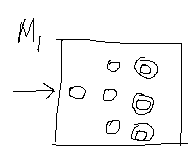
\includegraphics{2-5}
\end{center}

What does if mean for a word $W$ to be in $A_1^*$? %Take any finite number of strings, stick them all together, 
$W$ is in $A_1^*$ if we can break it up into pieces that are in the original language $A_1$.

\begin{center}
\includegraphics{diagrams/diags-2}
\end{center}

Every time we get to the an accept state of $M_1$, i.e. we've read a word in $A_1$ and we {\it might} want to start over. So we put $\ep$-transition leading from the accept state to the start state.

\begin{center}
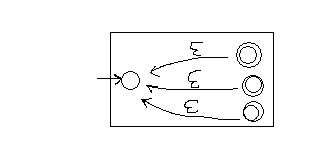
\includegraphics{2-7a}
\end{center}

As in the case with concatenation, we may not want to reset at the first cut point, because maybe there is no way to cut remaining piece into words in $A_1$. So every time get to an accept, have the \emph{choice} to restart---we split into 2 threads, one that looks to continue the current word, and one that restarts.
%Option to restart, can keep doing what.

There is a slight problem: we need to accept the empty string as well. %might be other reasons in start state. 

To do this we add a new start state, and add an $\ep$-transition to the old start state. Then we're good.

\begin{center}
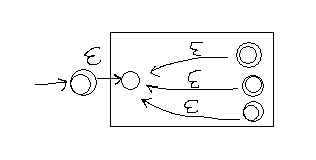
\includegraphics{2-7b}
\end{center} 
\end{proof}

NFA's also give us an easier way to prove closure under union.

\begin{proof}[Proof of closure under $\cup$]
Suppose we're given $M_1$ recognizing $A_1$ and $M_2$ recognizing $A_2$. To build $M$ recognizing $A_1$ and $A_2$, it needs to go through $M_1$ and $M_2$ in parallel. So we put the two machines together, add a new start state, and have it branch by $\ep$-transitions to the start states {\it both} $M_1$ and $M_2$. This way we'll have a finger in $M_1$ and a finger in $M_2$ at the same time.

\begin{center}
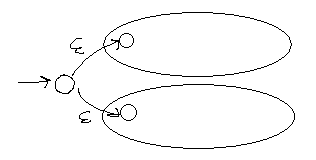
\includegraphics{2-11}
\end{center} 
\end{proof}

\subsection{Converting a finite automaton into a regular expression}
The proof of the closure properties gives us a procedure for converting a regular expression into finite automaton. This procedure comes right out of the construction of machines for $\cup$, $\circ$, and ${}^*$. This will prove part 2 of Theorem~\ref{thm:regex-FA}.
%thm: every regular expression $R$ has an equivalent DFA M.

We do a proof by example: consider $(ab\cup a^*)$. We convert this to a finite automaton as follows. %inductive proof
For $a,b$ we make the following automata. 

\begin{center}
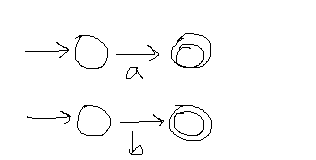
\includegraphics[scale=0.5]{2-8}
\end{center} 

We build up our expression from small pieces and then combine. Let's make an automaton for $ab$. We use our construction for closure under concatenation.

\begin{center}
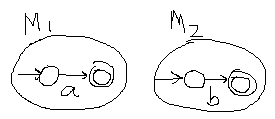
\includegraphics{2-9}\\

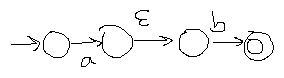
\includegraphics{2-10a}
\end{center} 

This machine recognizes $ab$. Now we do $a^*$.

\begin{center}
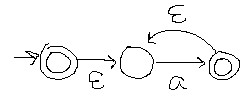
\includegraphics{2-10b}
\end{center} 

%(Closure under union can be proved with nondeterminism, combine with new start state, branching with start state under $\ep$, Fig 11.)
Finally we put the FA's for $ab$ and $a^*$ together, using the $\cup$ construction, to get the FA recognizing $ab\cup a^*$.

\begin{center}
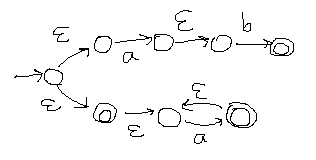
\includegraphics[scale=0.75]{2-10c}
\end{center} 

\cpbox{The constructions for $\cup$, $\circ$, and ${}^{*}$ give a way to construct a FA for any regular expression.}